\documentclass[tikz,border=3mm]{standalone}
\usepackage{pgfplots}
\pgfplotsset{compat=1.18}
\begin{document}
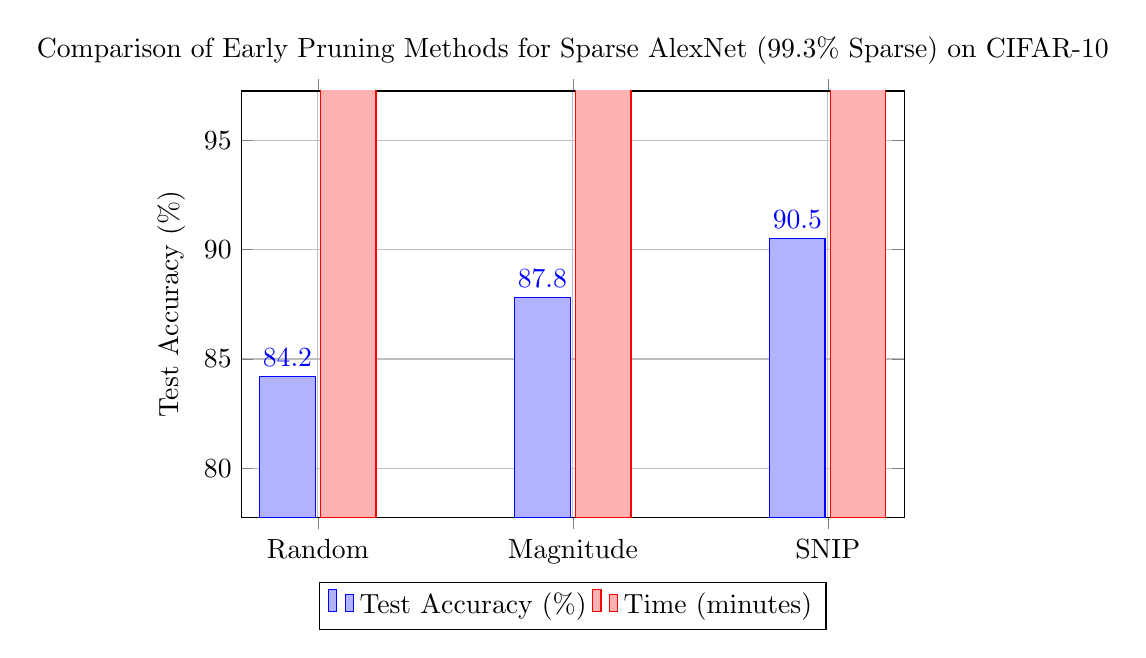
\begin{tikzpicture}
    \begin{axis}[
        ybar,
        bar width=20pt,
        enlargelimits=0.15,
        ylabel={Test Accuracy (\%)},
        xlabel={Early Pruning Method},
        symbolic x coords={Random, Magnitude, SNIP},
        xtick=data,
        nodes near coords,
        nodes near coords align={vertical},
        ymin=80, ymax=95,
        grid=major,
        legend style={at={(0.5,-0.15)}, anchor=north, legend columns=-1},
        width=10cm,
        height=7cm,
        title={Comparison of Early Pruning Methods for Sparse AlexNet (99.3\% Sparse) on CIFAR-10},
    ]
    % Data: Method | Time (minutes) | Accuracy (%)
    \addplot coordinates {
        (Random, 84.2)
        (Magnitude, 87.8)
        (SNIP, 90.5)
    };
    \addplot coordinates {
        (Random, 120)
        (Magnitude, 115)
        (SNIP, 108)
    };
    \legend{Test Accuracy (\%), Time (minutes)}
    \end{axis}
\end{tikzpicture}
\end{document}